\documentclass{beamer}

%%%%%%%%%%%%%Solarized Theme%%%%%%%%%%%%%%%
\usecolortheme[dark,accent=cyan]{solarized}
\beamertemplatenavigationsymbolsempty
%%%%%Packages%%%%%
\usefonttheme{serif}
\usepackage[T1]{fontenc}
\usepackage[utf8]{inputenc}
\usepackage[english]{babel}
\usepackage{fontawesome}
\usepackage{minted}

\definecolor{DarkGray}{gray}{0.1}
\usemintedstyle{paraiso-dark}


\usepackage{graphicx}
\usepackage{hyperref}
\usepackage{colortbl, xcolor}
\usepackage{booktabs}
\usepackage{amsmath,amsthm, amssymb, latexsym}

\usepackage{tikz}
\usepackage{standalone}
\usepackage{siunitx}
\usetikzlibrary{calc, positioning, arrows, arrows.meta, shapes}

\begin{document}

\begin{frame}
    \begin{center}
        \LARGE{\textbf{\textcolor{orange}{Gaining from \& giving to the community}}} \\

        \vspace{1cm}
        \normalsize{@NikoletaGlyn}

    \end{center}
\end{frame}

\begin{frame}
    \begin{center}
    
\includegraphics[width=0.24\textwidth]{static/cardiff_uni_logo.png}\hspace{6pt}
    
\includegraphics[width=0.24\textwidth, height=0.245\textwidth]{static/django_girls.png}\vspace{10pt}

    
\includegraphics[width=0.24\textwidth]{static/ssi-logo.png} \hspace{6pt}
    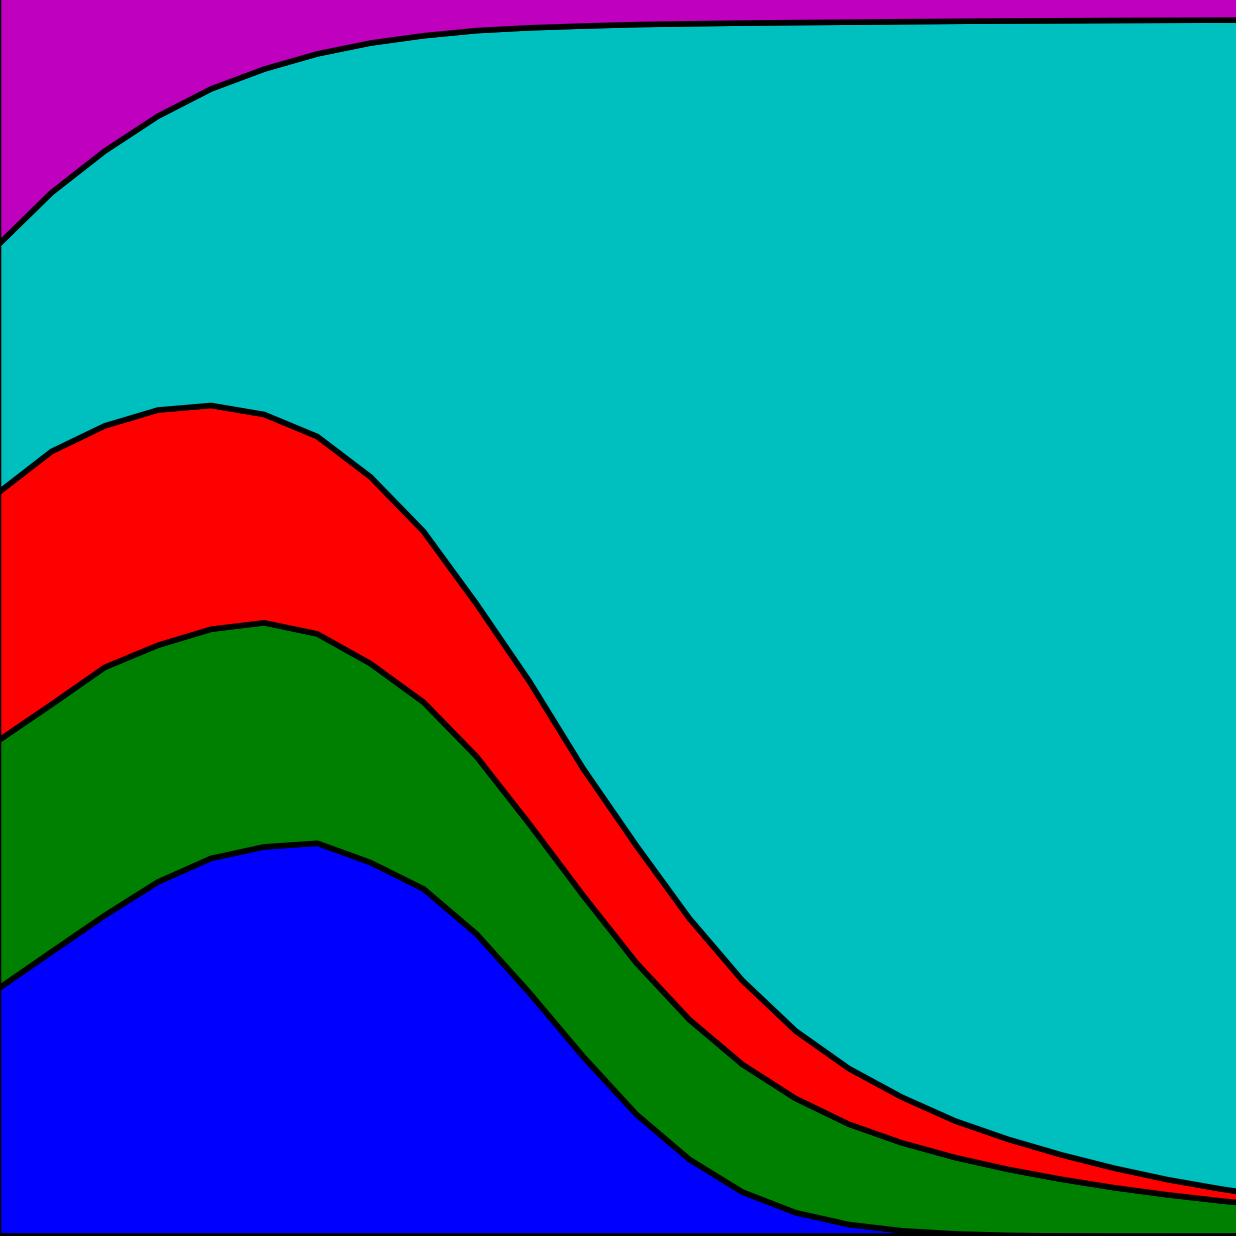
\includegraphics[width=0.24\textwidth]{static/axelrod-logo.png}

    \end{center}
\end{frame}

\begin{frame}
    \centering
    
\includegraphics[width=.2\textwidth]{static/players} \hspace{.6cm}
    
\includegraphics[width=.2\textwidth]{static/actions} \hspace{.6cm}
    
\includegraphics[width=.2\textwidth]{static/objective}
\end{frame}

\begin{frame}
    \begin{center}
    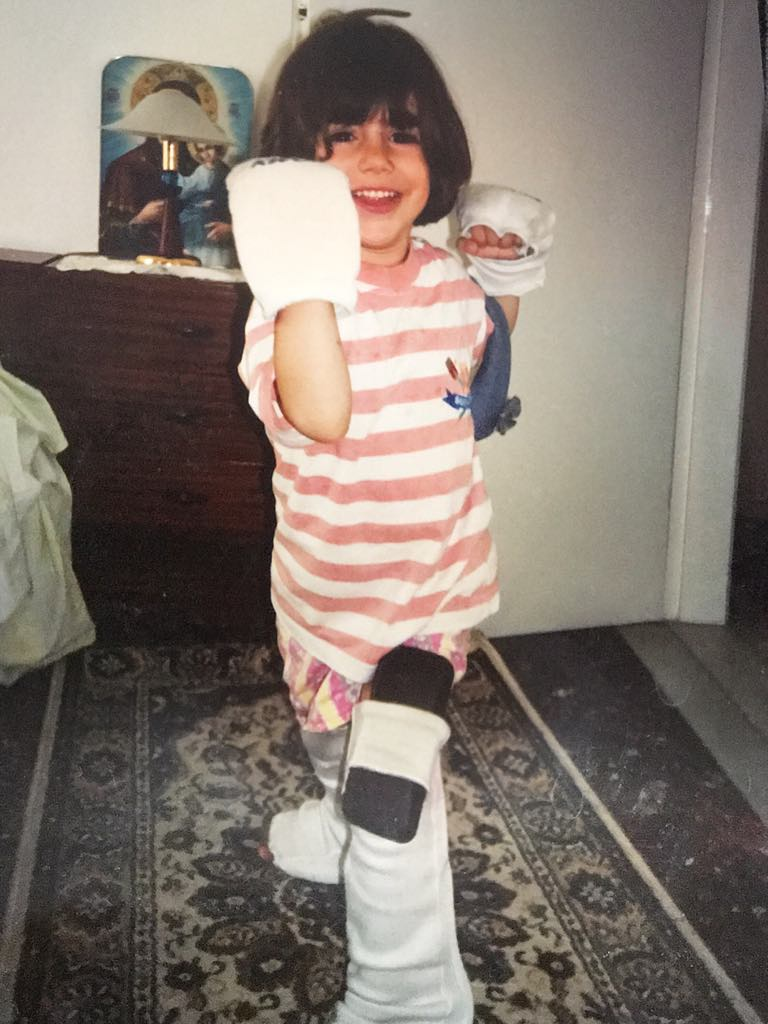
\includegraphics[width=.6\textwidth]{static/young_me}
    \end{center}
\end{frame}

\begin{frame}
    \begin{center}
    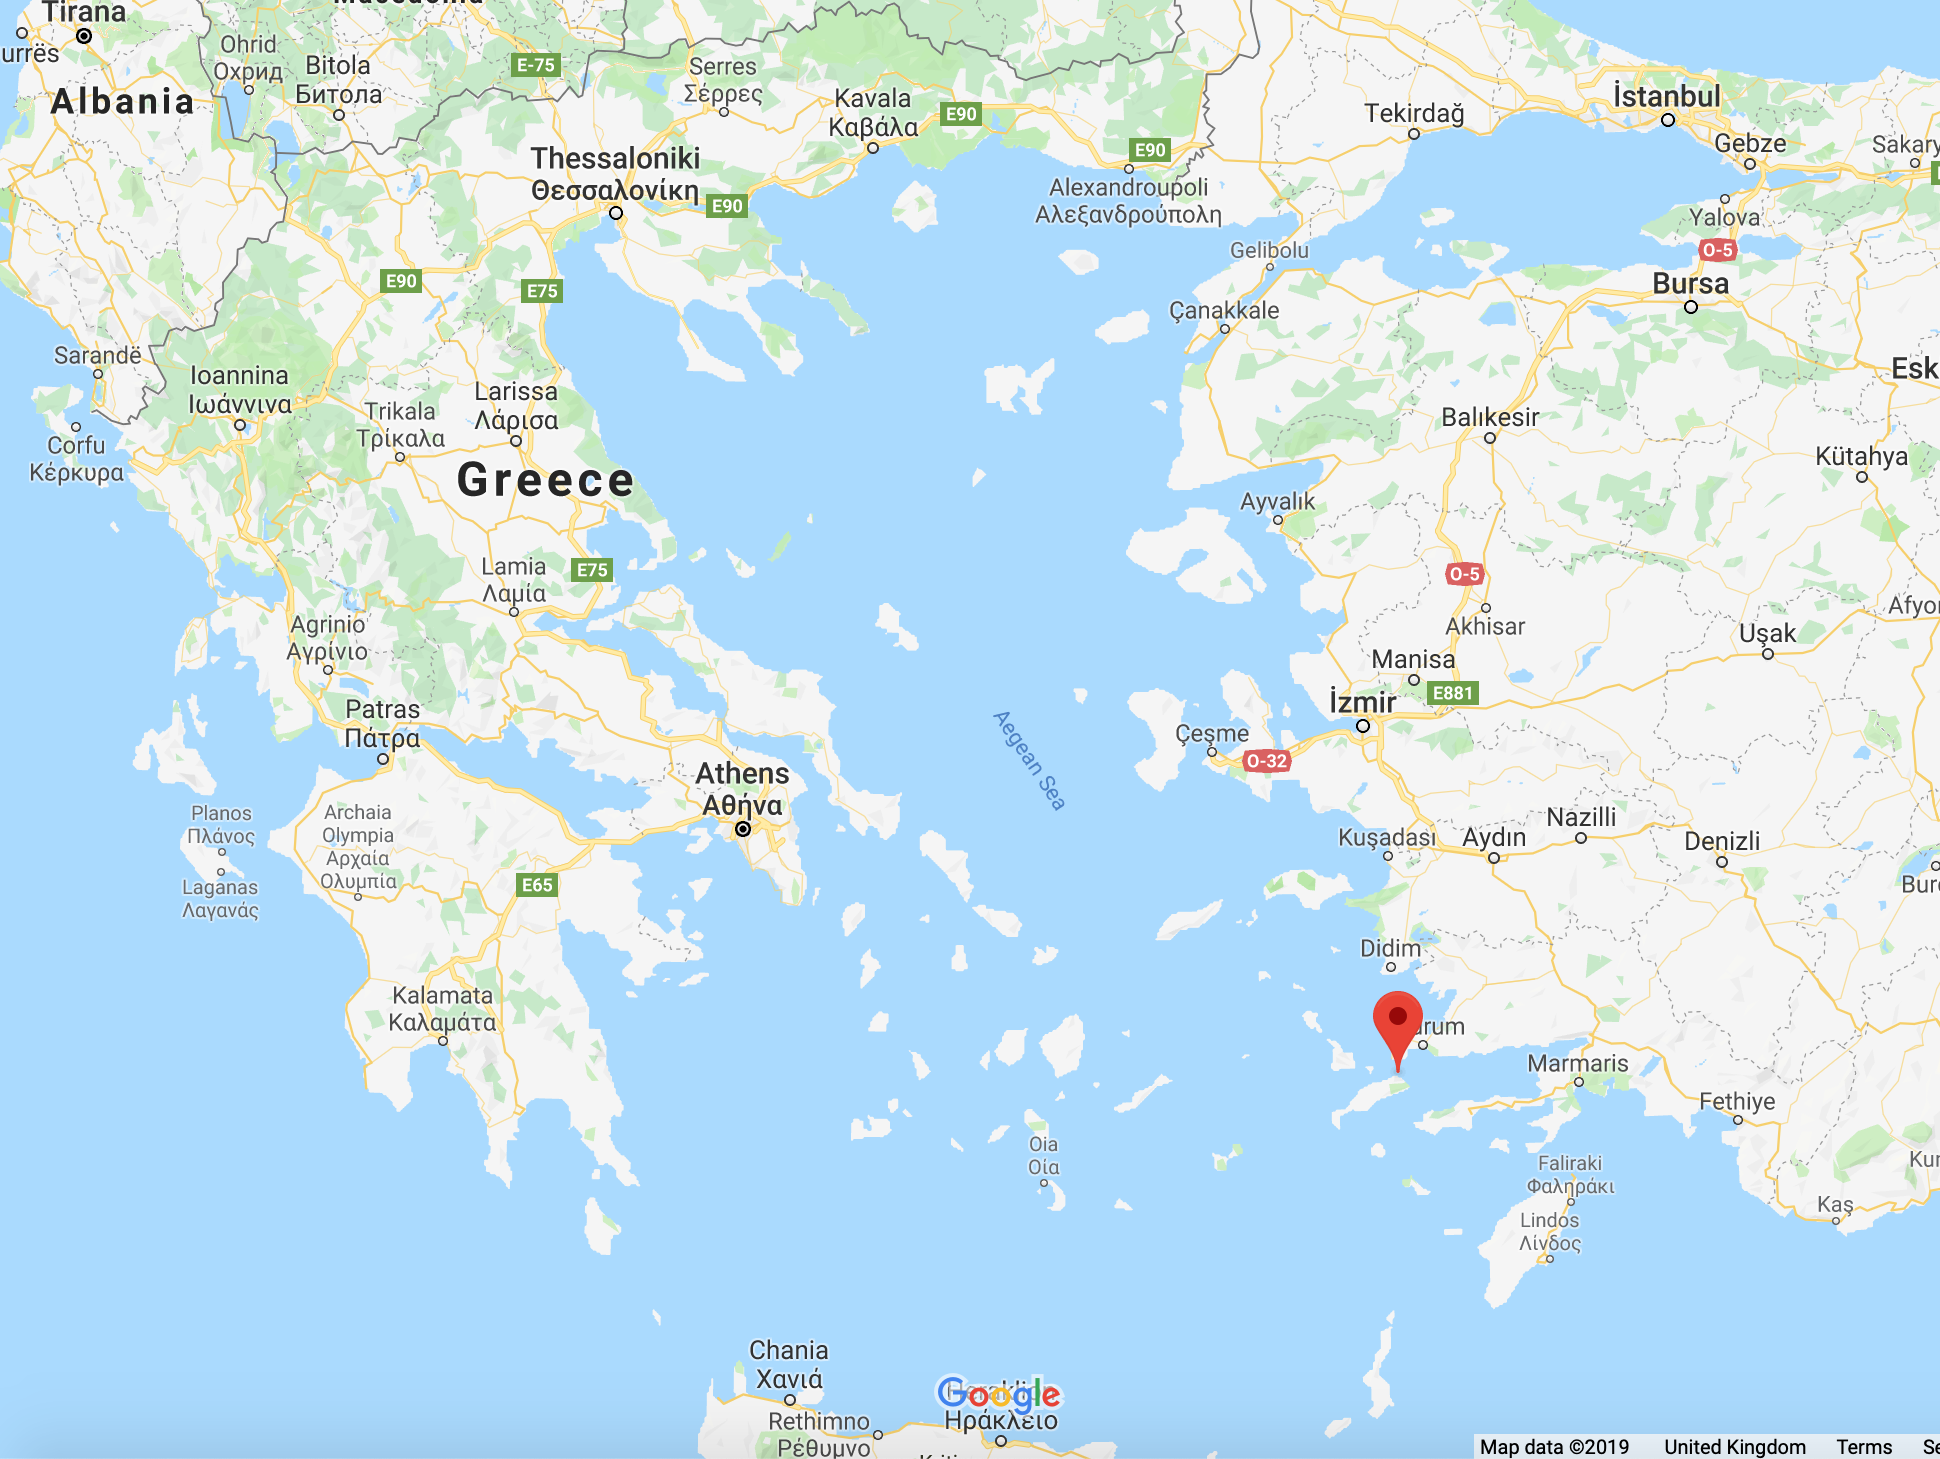
\includegraphics[width=.7\textwidth]{static/kos}
    \end{center}
\end{frame}

\begin{frame}
    \begin{center}
    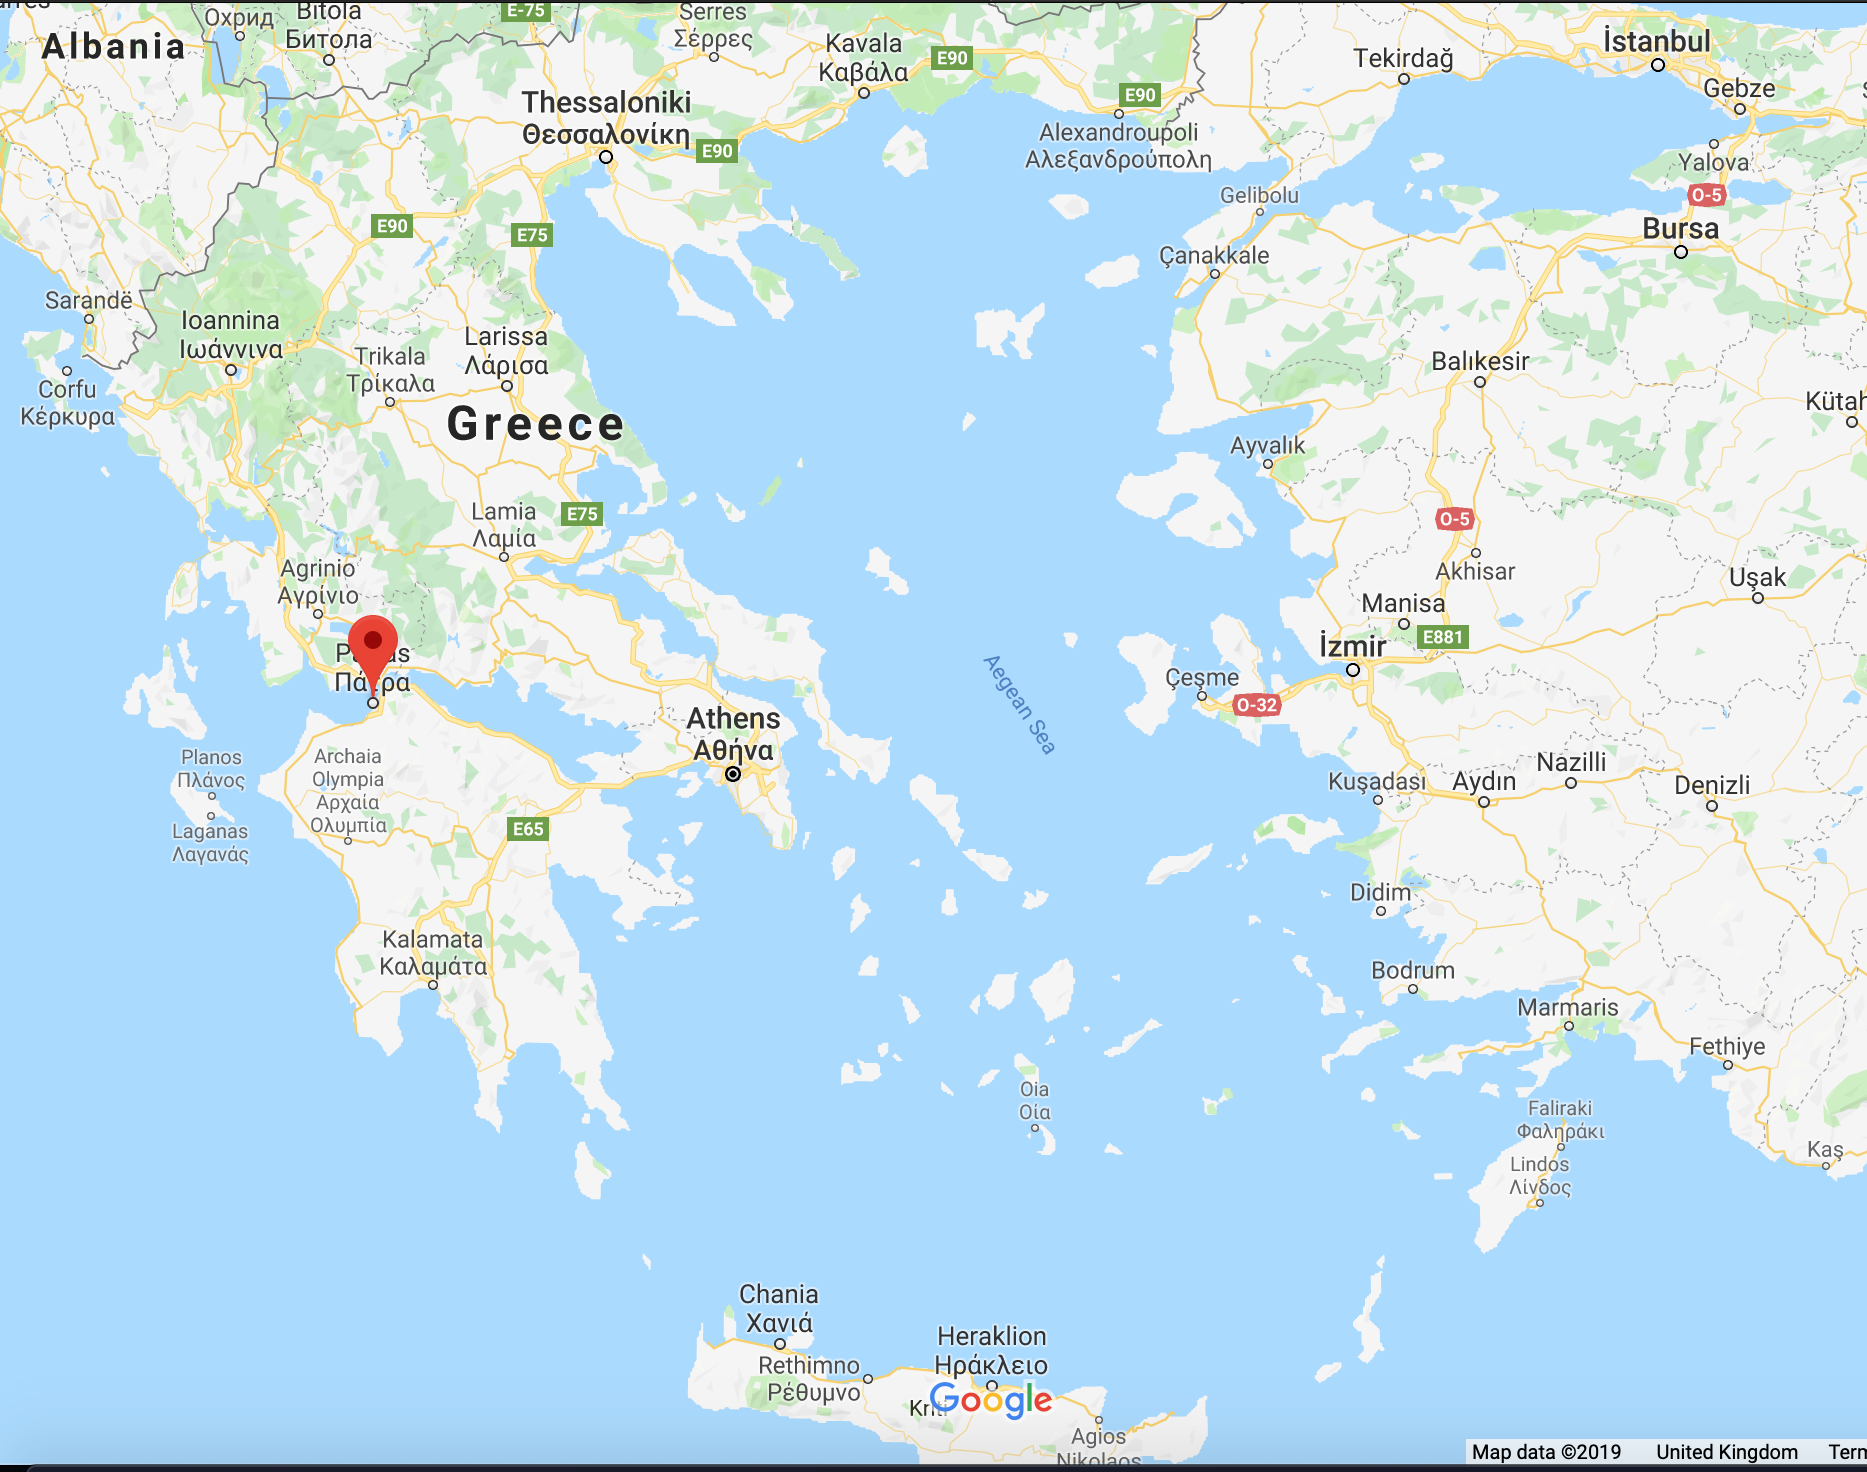
\includegraphics[width=.7\textwidth]{static/patras}
    \end{center}
\end{frame}

\begin{frame}
    \begin{center}
    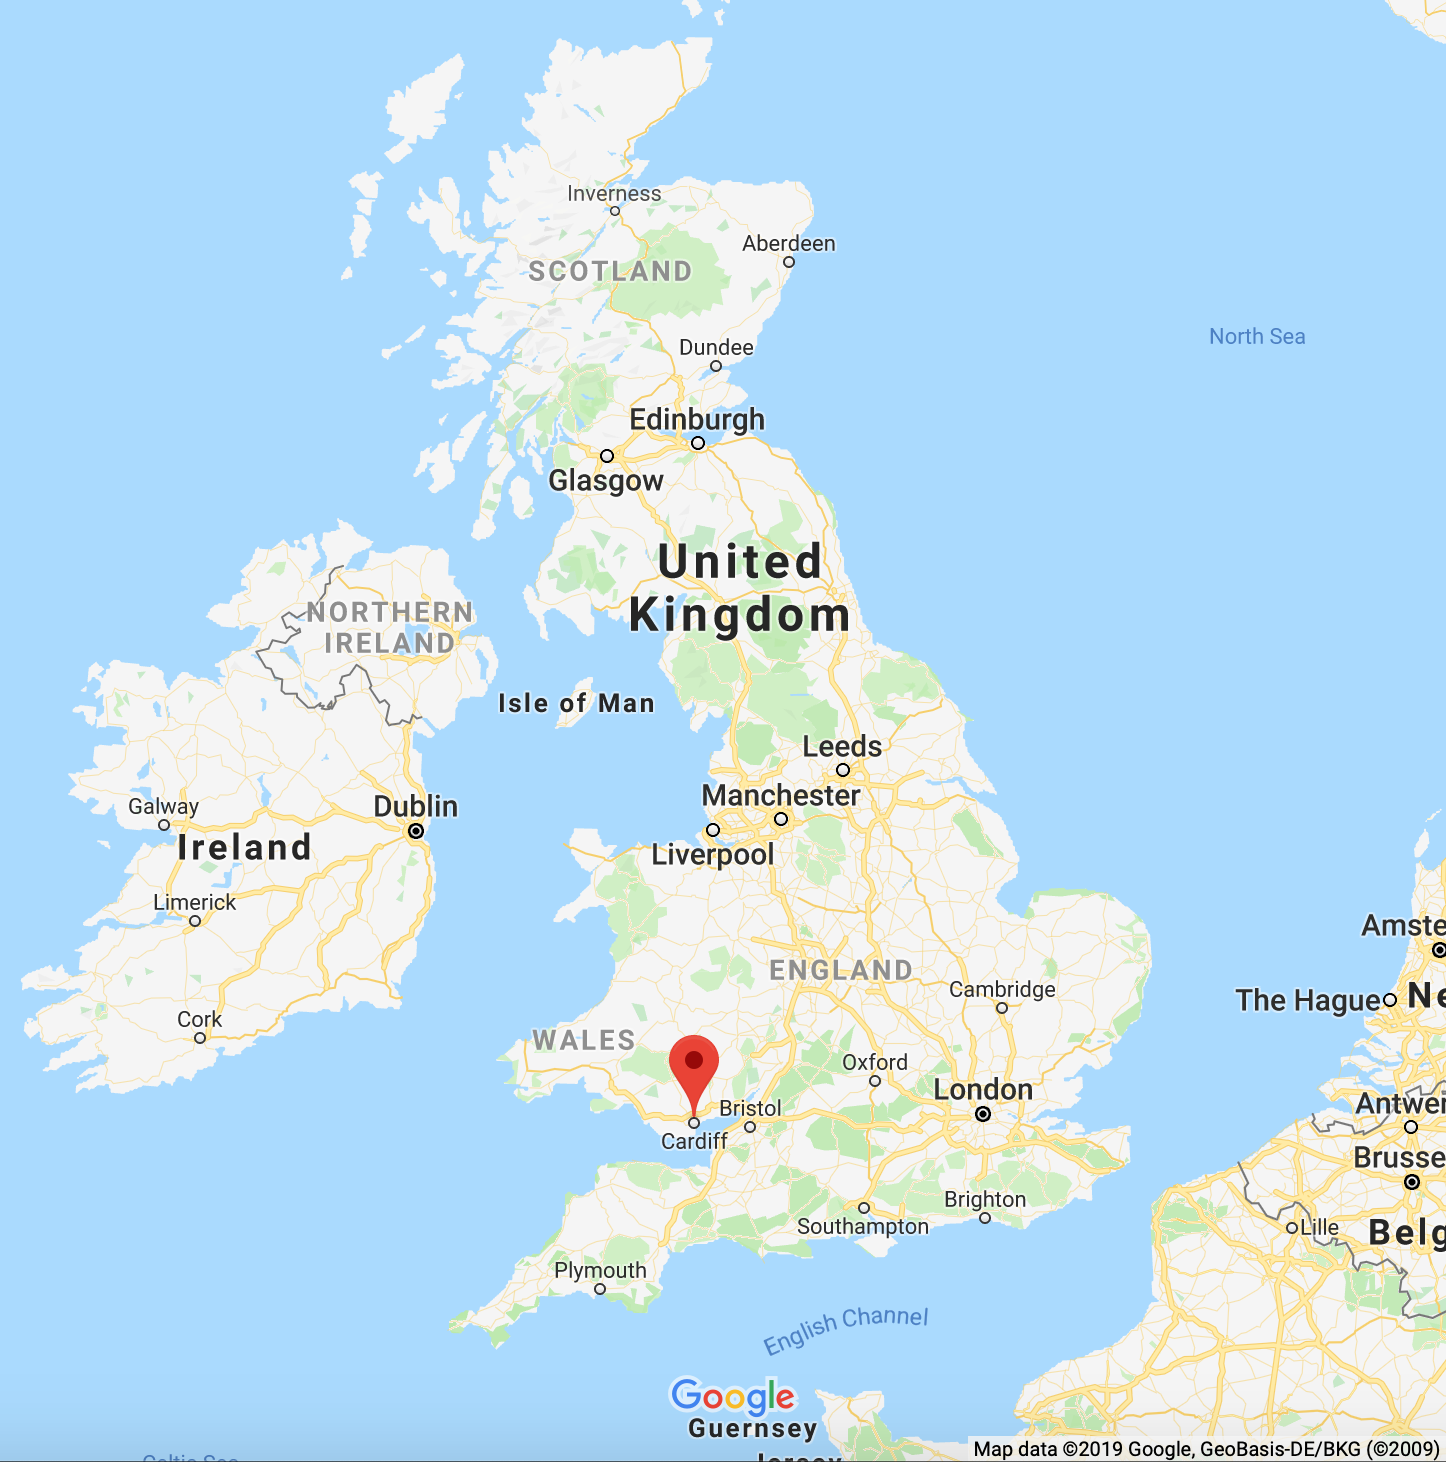
\includegraphics[width=.7\textwidth]{static/cardiff}
    \end{center}
\end{frame}

\begin{frame}
    \begin{center}
    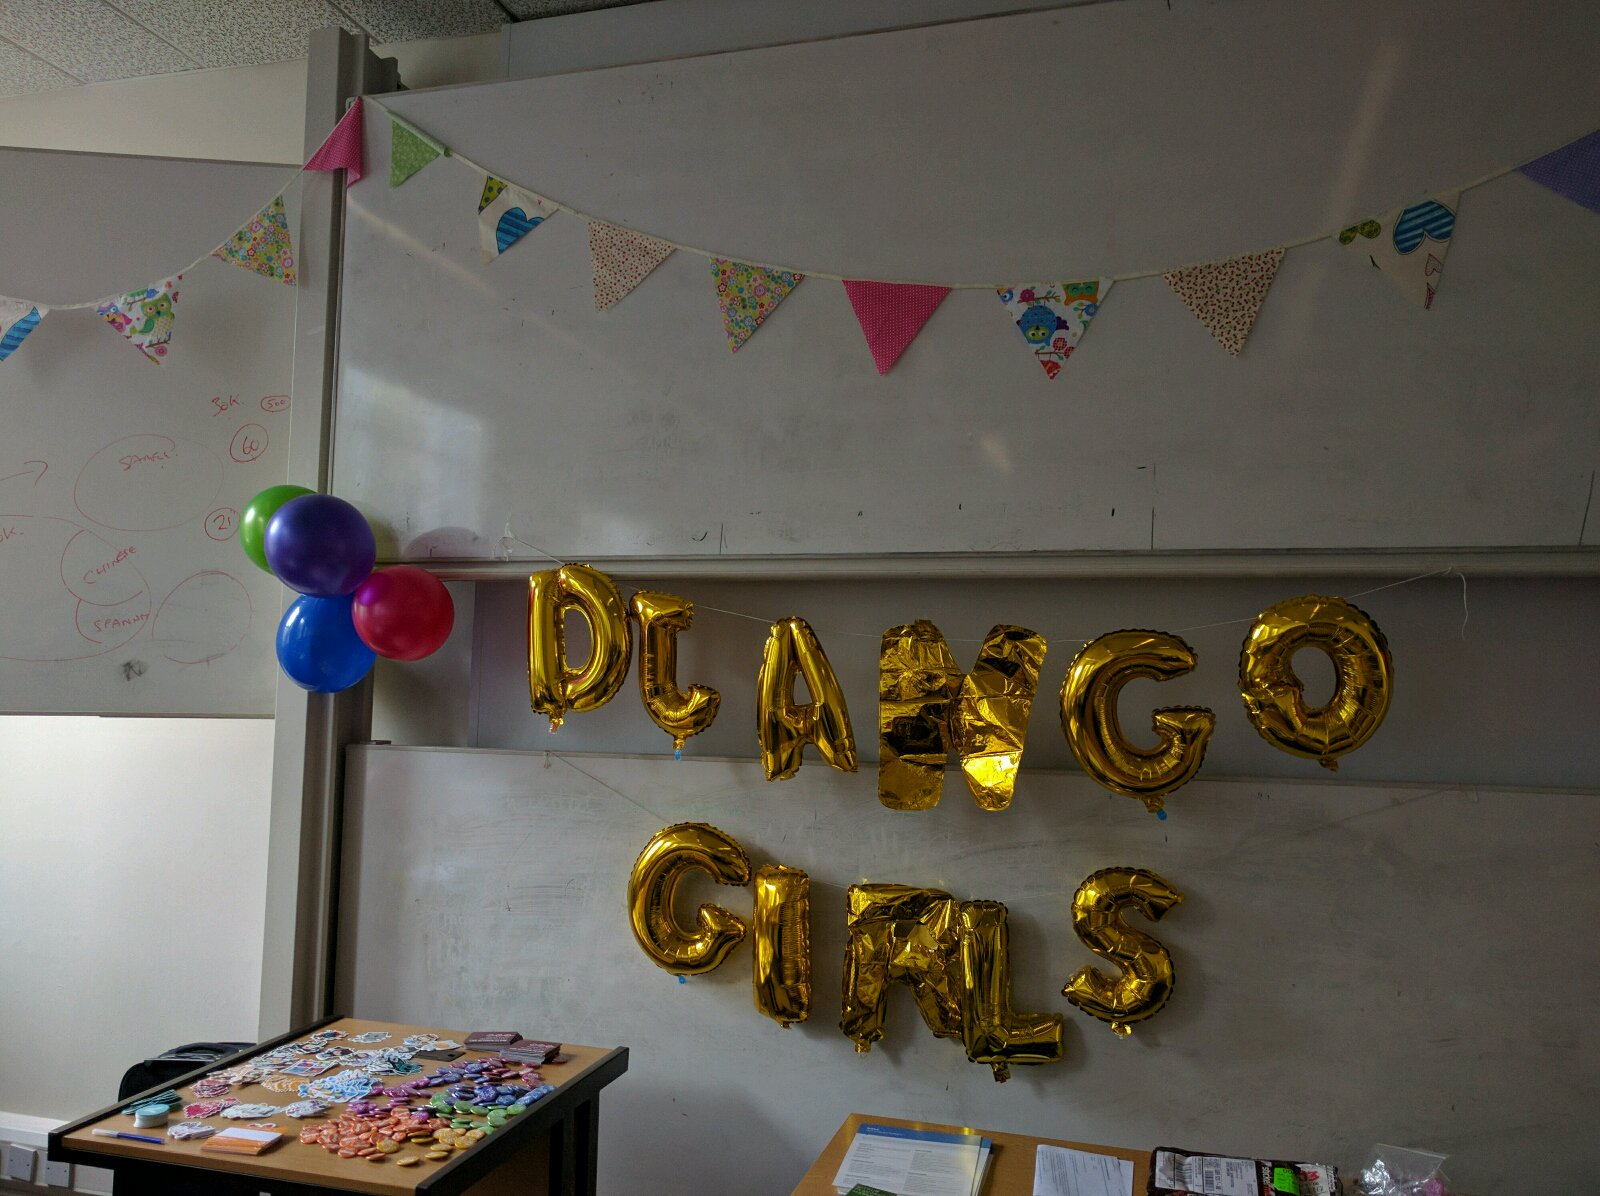
\includegraphics[width=.7\textwidth]{static/first_django_girls.jpeg} \\
    \textbf{CARDIFF 2016}
    \end{center}
\end{frame}

\begin{frame}
    \centering
    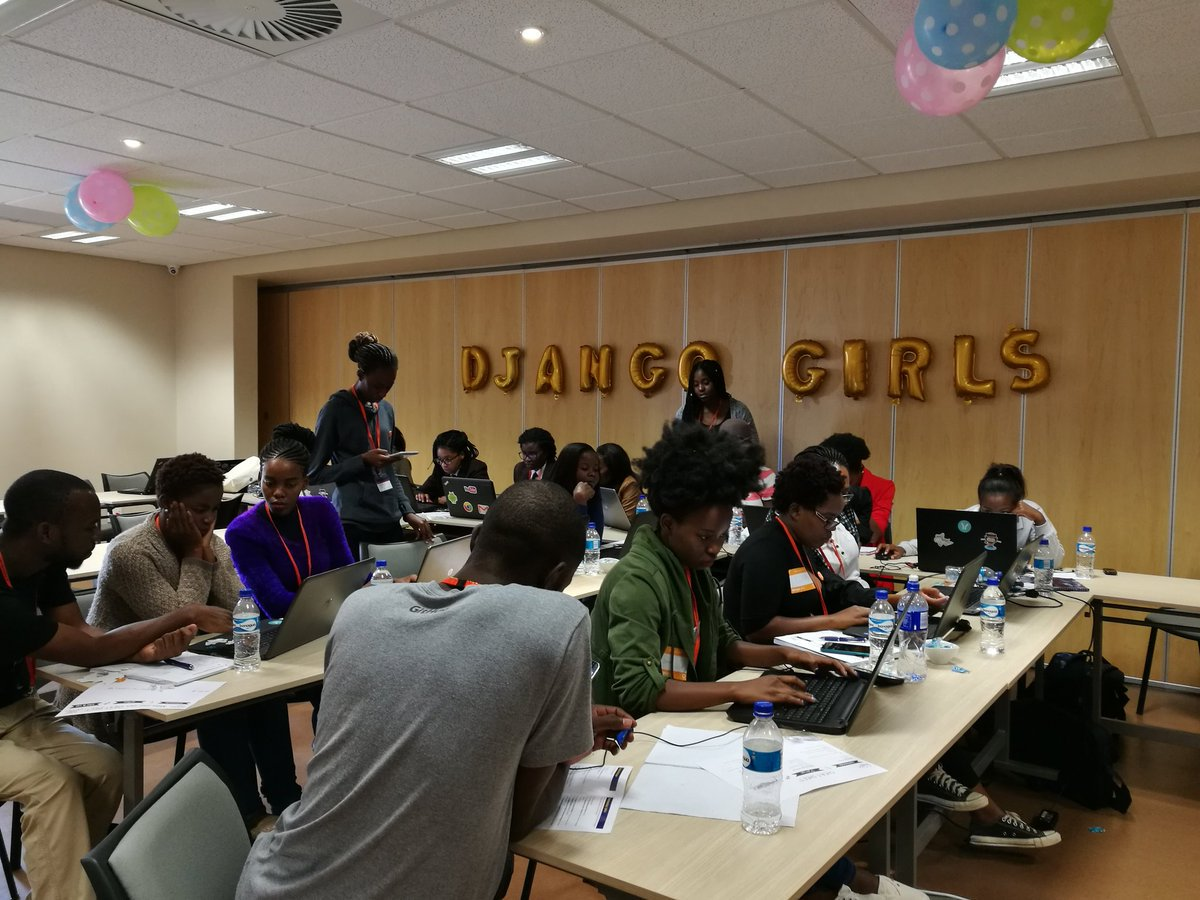
\includegraphics[width=.7\textwidth]{static/windhoek_2017} \\
    \textbf{WINDHOEK 2017}
\end{frame}

\begin{frame}
    \centering
    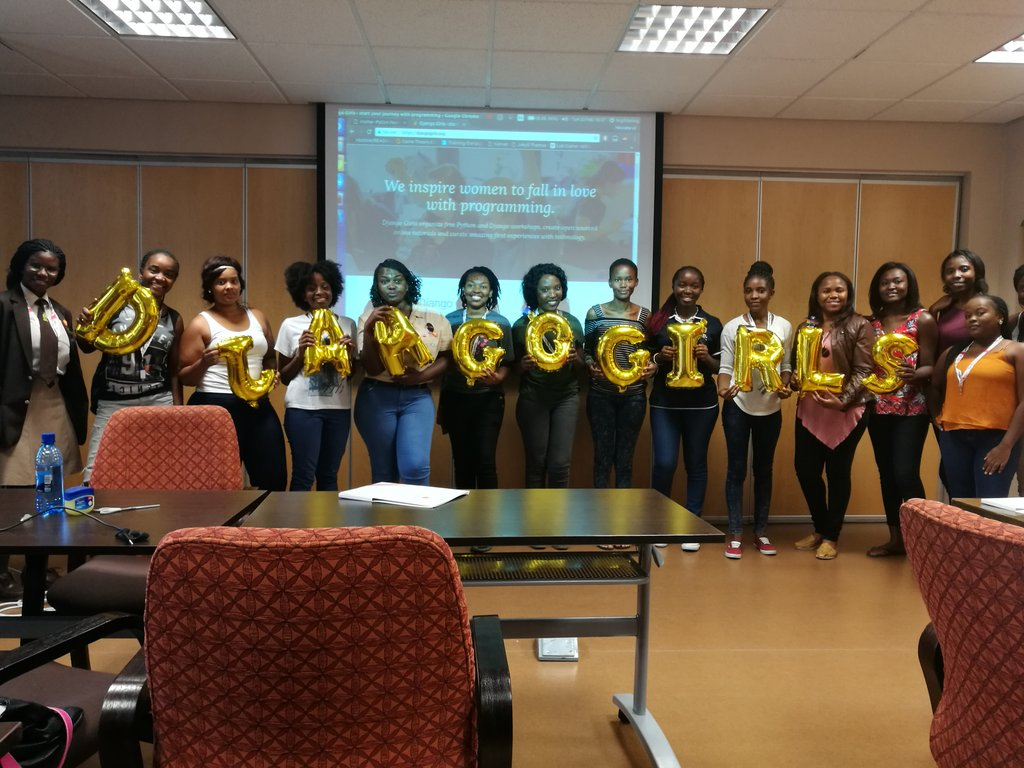
\includegraphics[width=.7\textwidth]{static/windhoek_2018} \\
    \textbf{WINDHOEK 2018}
\end{frame}

\begin{frame}
        \centering
    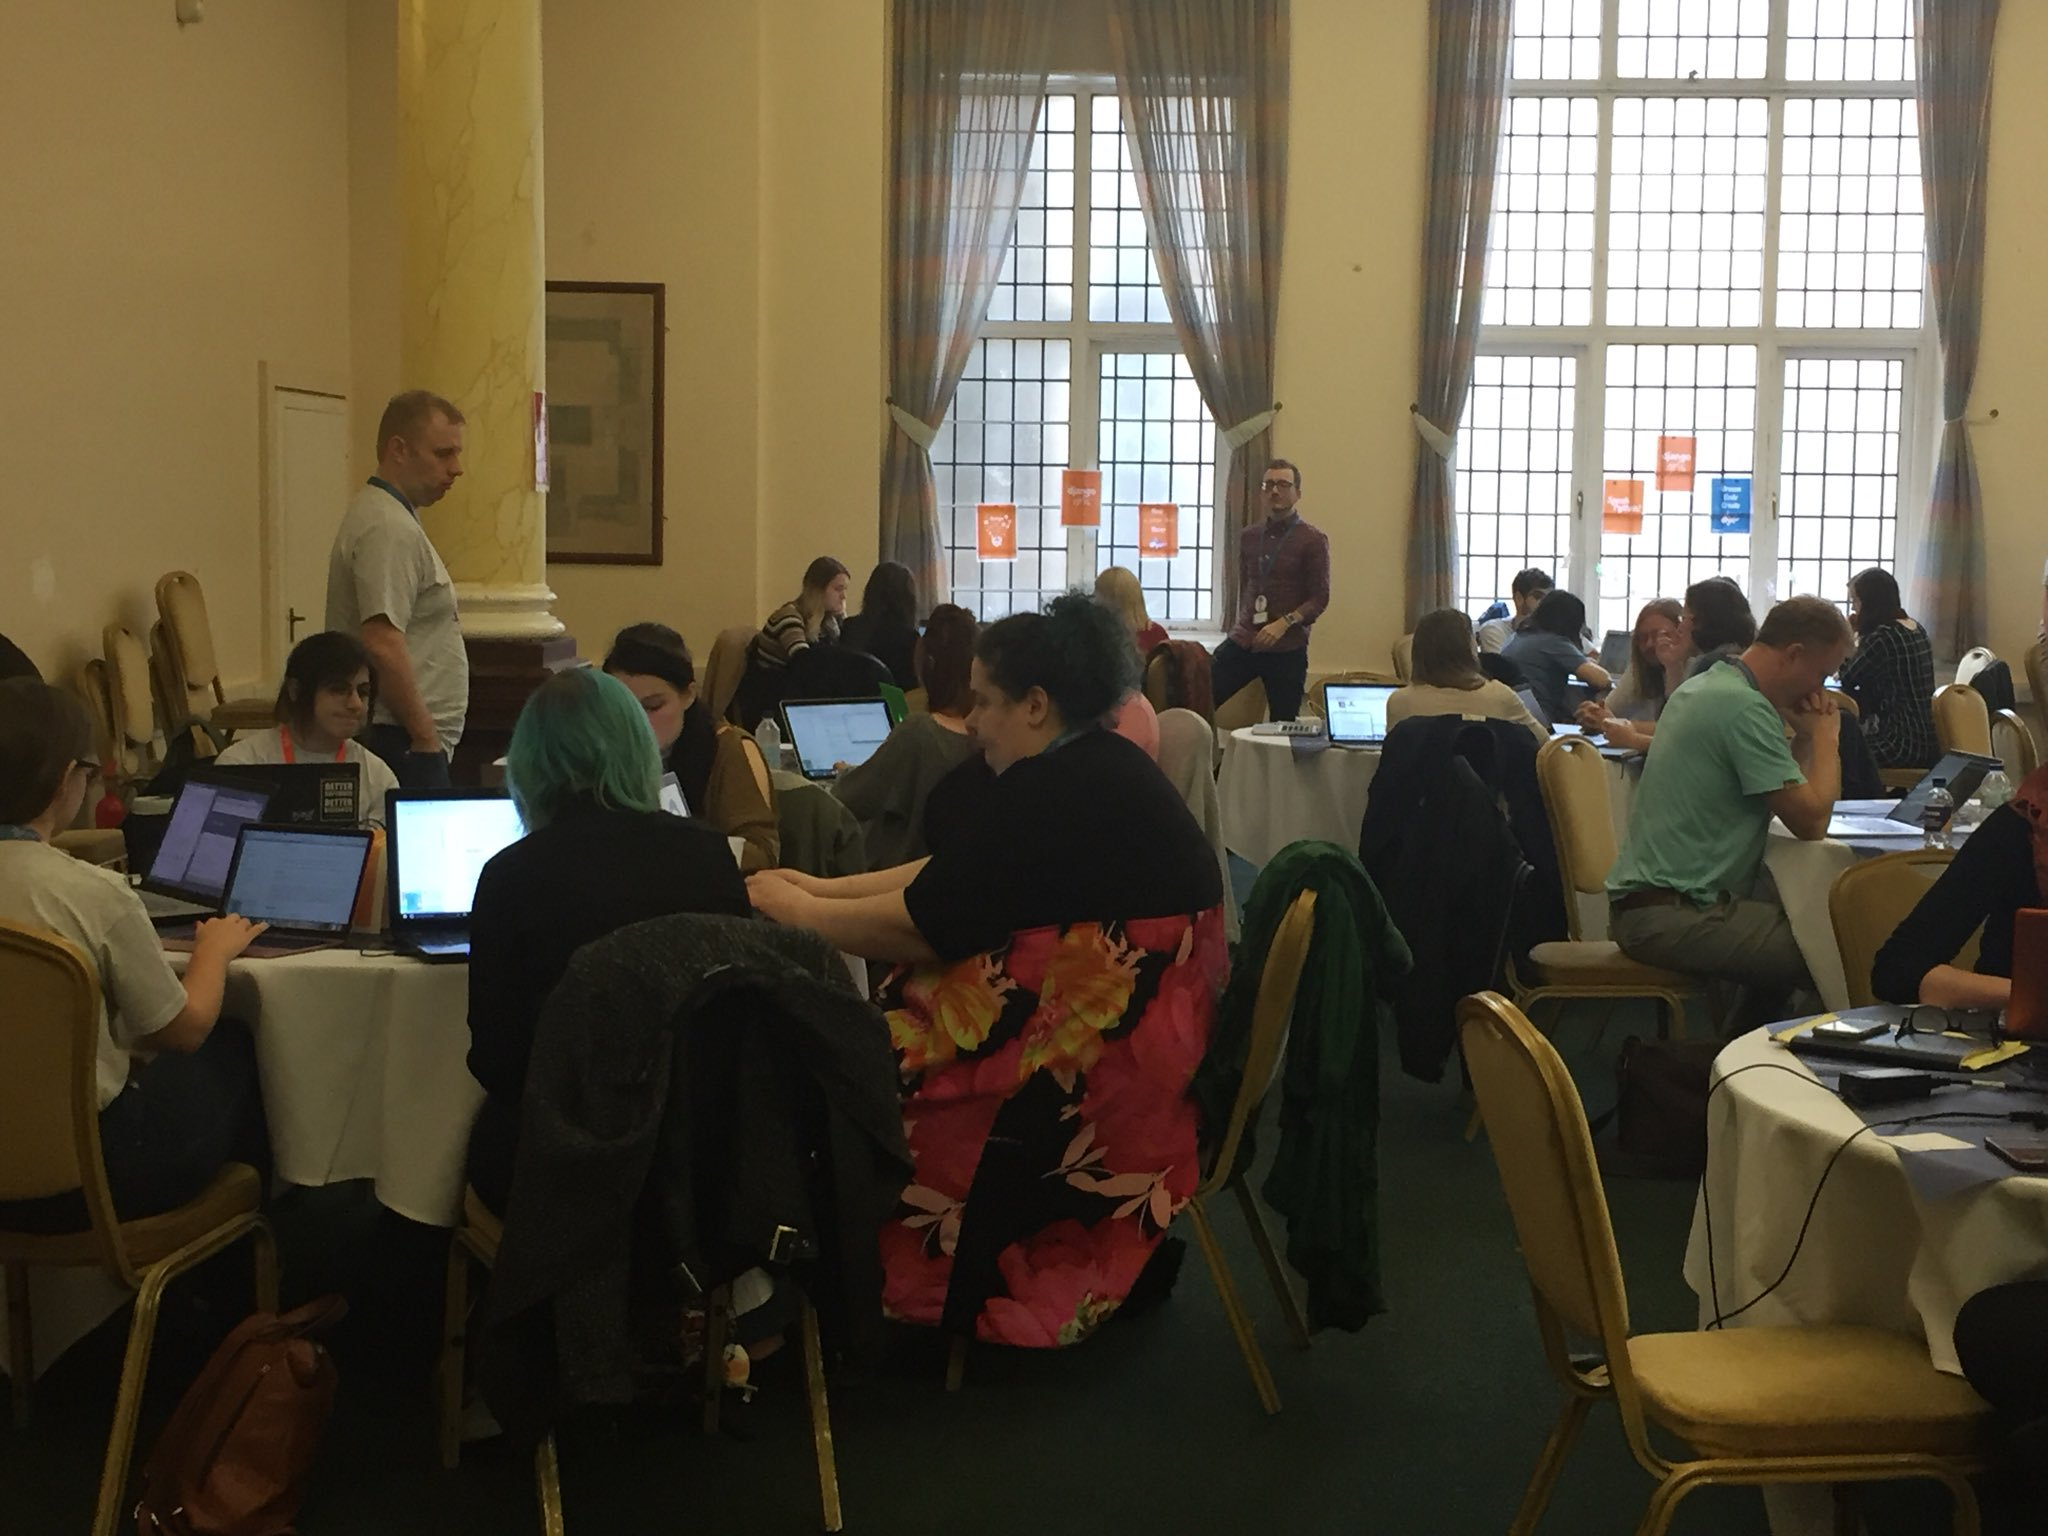
\includegraphics[width=.7\textwidth]{static/cardiff_2017} \\
    \textbf{CARDIFF 2017}
\end{frame}

\begin{frame}
    \centering
    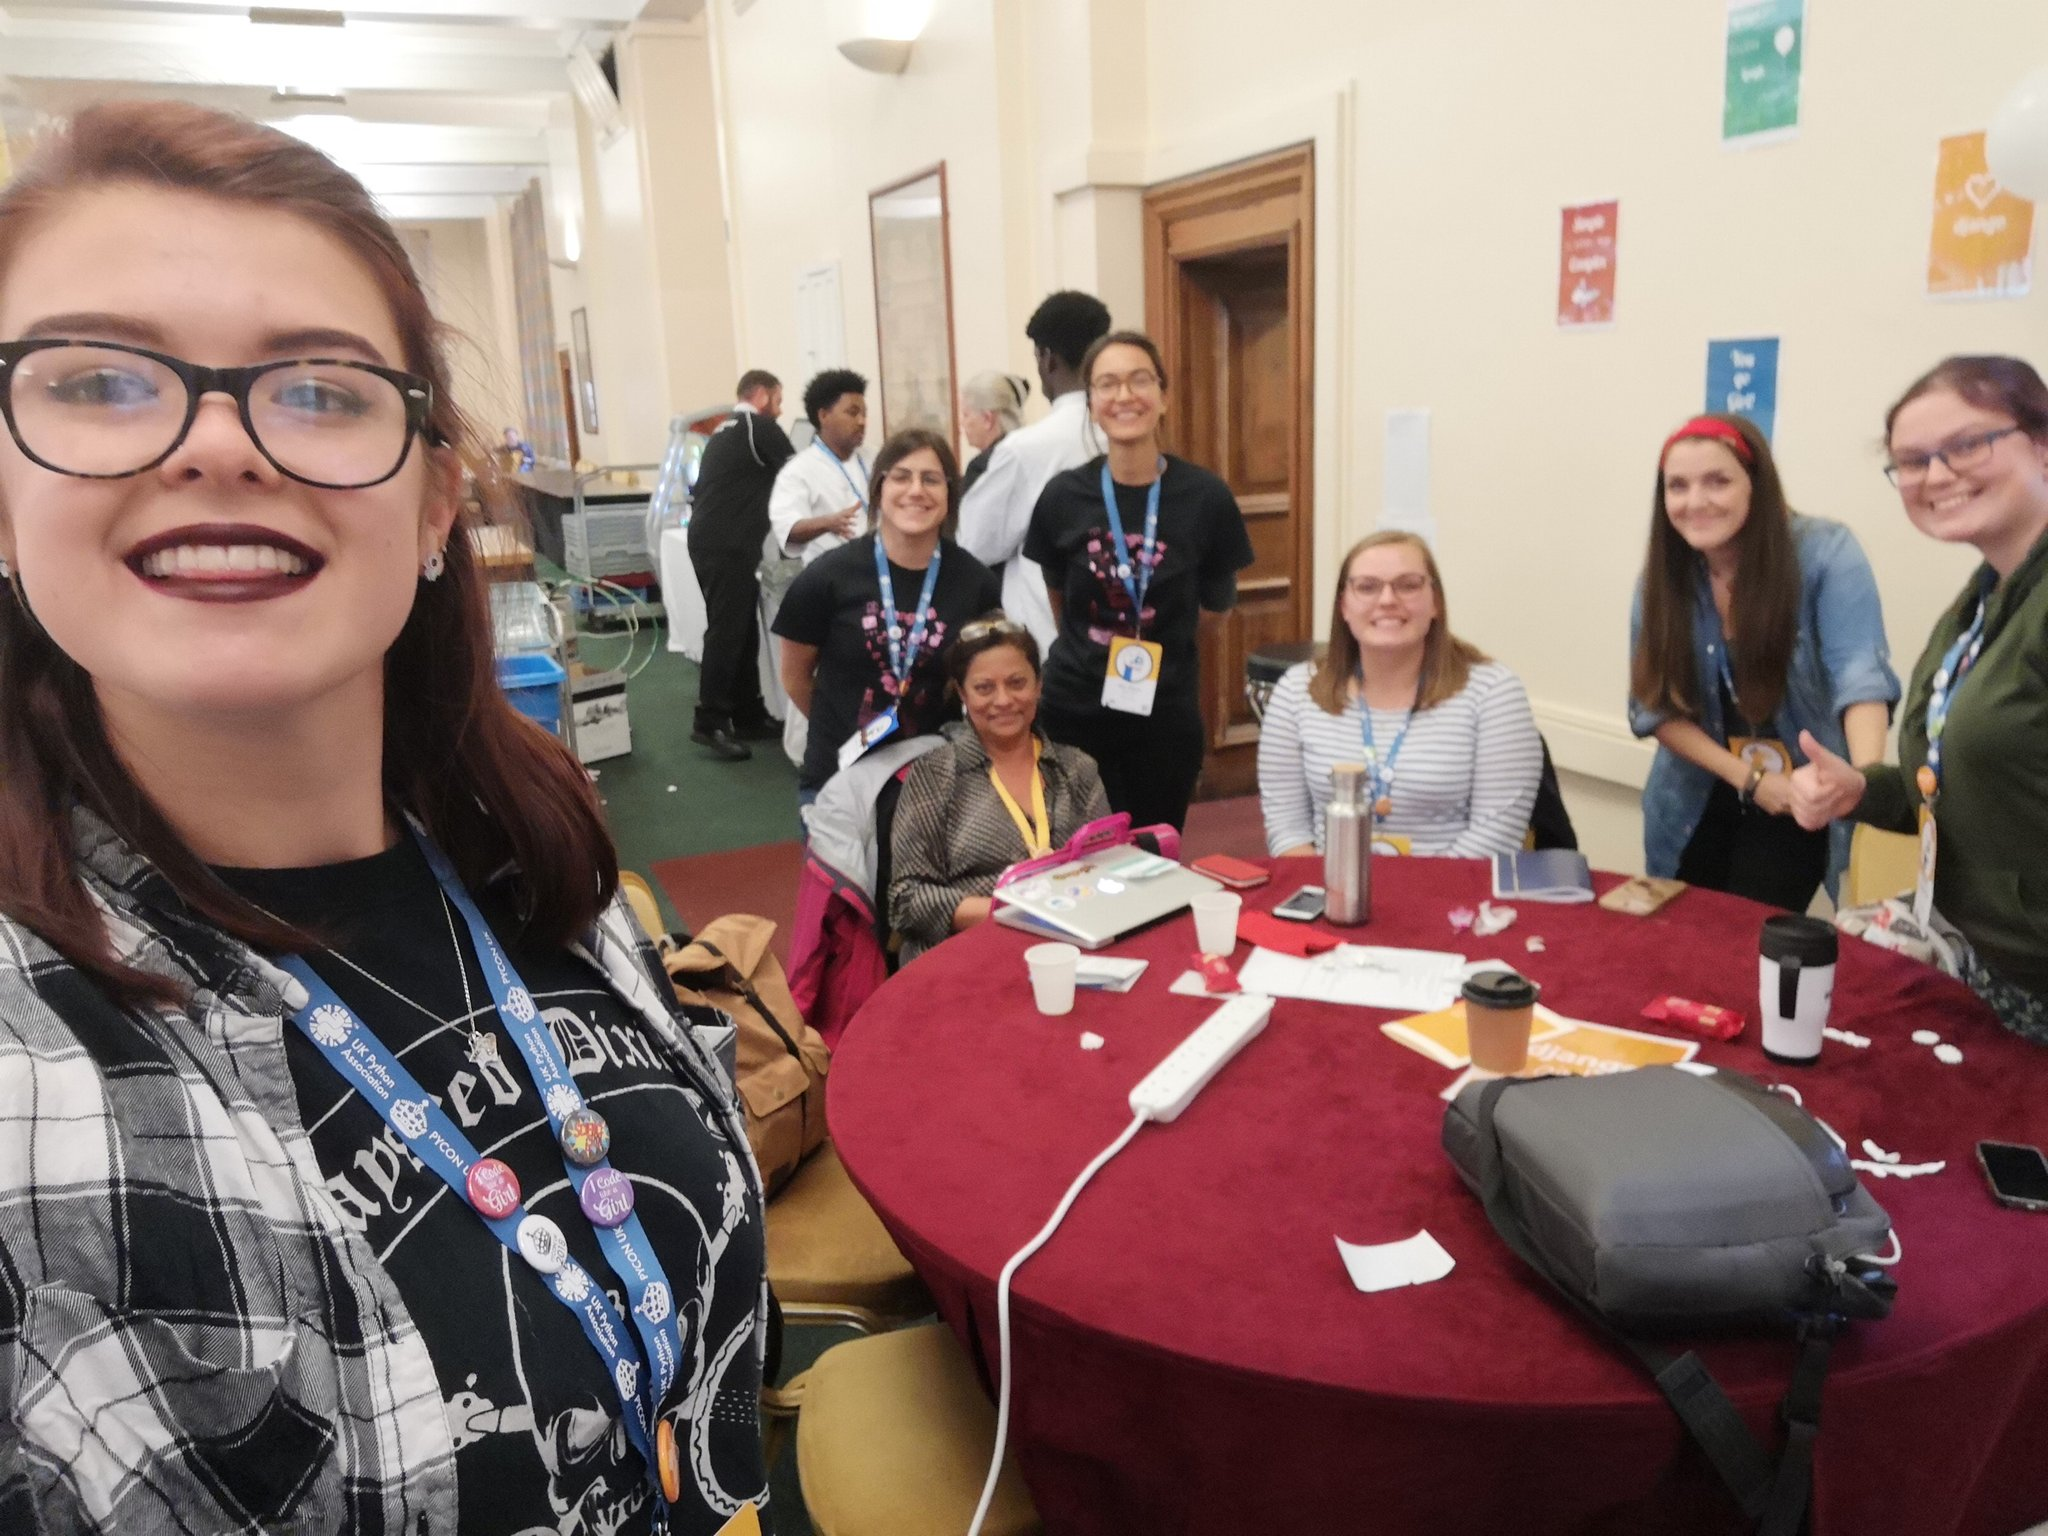
\includegraphics[width=.7\textwidth]{static/cardiff_2018} \\
    \textbf{CARDIFF 2018}
\end{frame}

\begin{frame}
    \begin{center}
    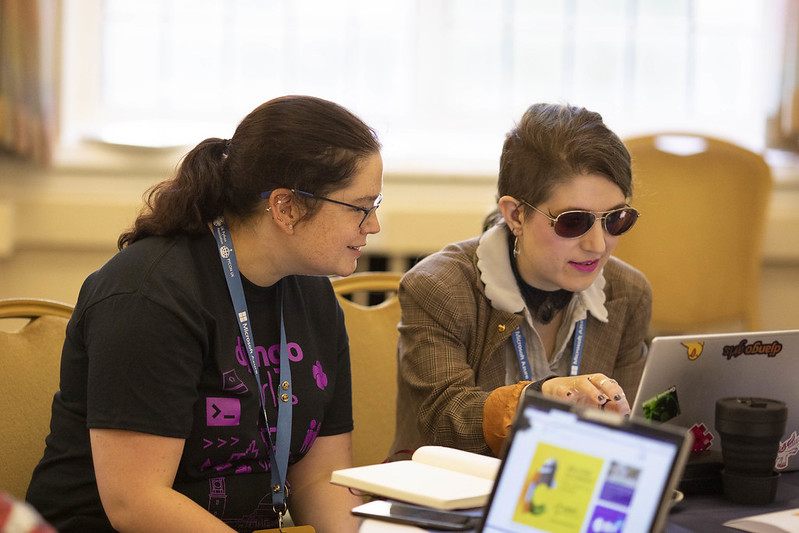
\includegraphics[width=.7\textwidth]{static/coach} \\
    \textbf{CARDIFF 2019 - Tamsin @deltabug}
    \end{center}
\end{frame}

\begin{frame}
    \begin{center}
        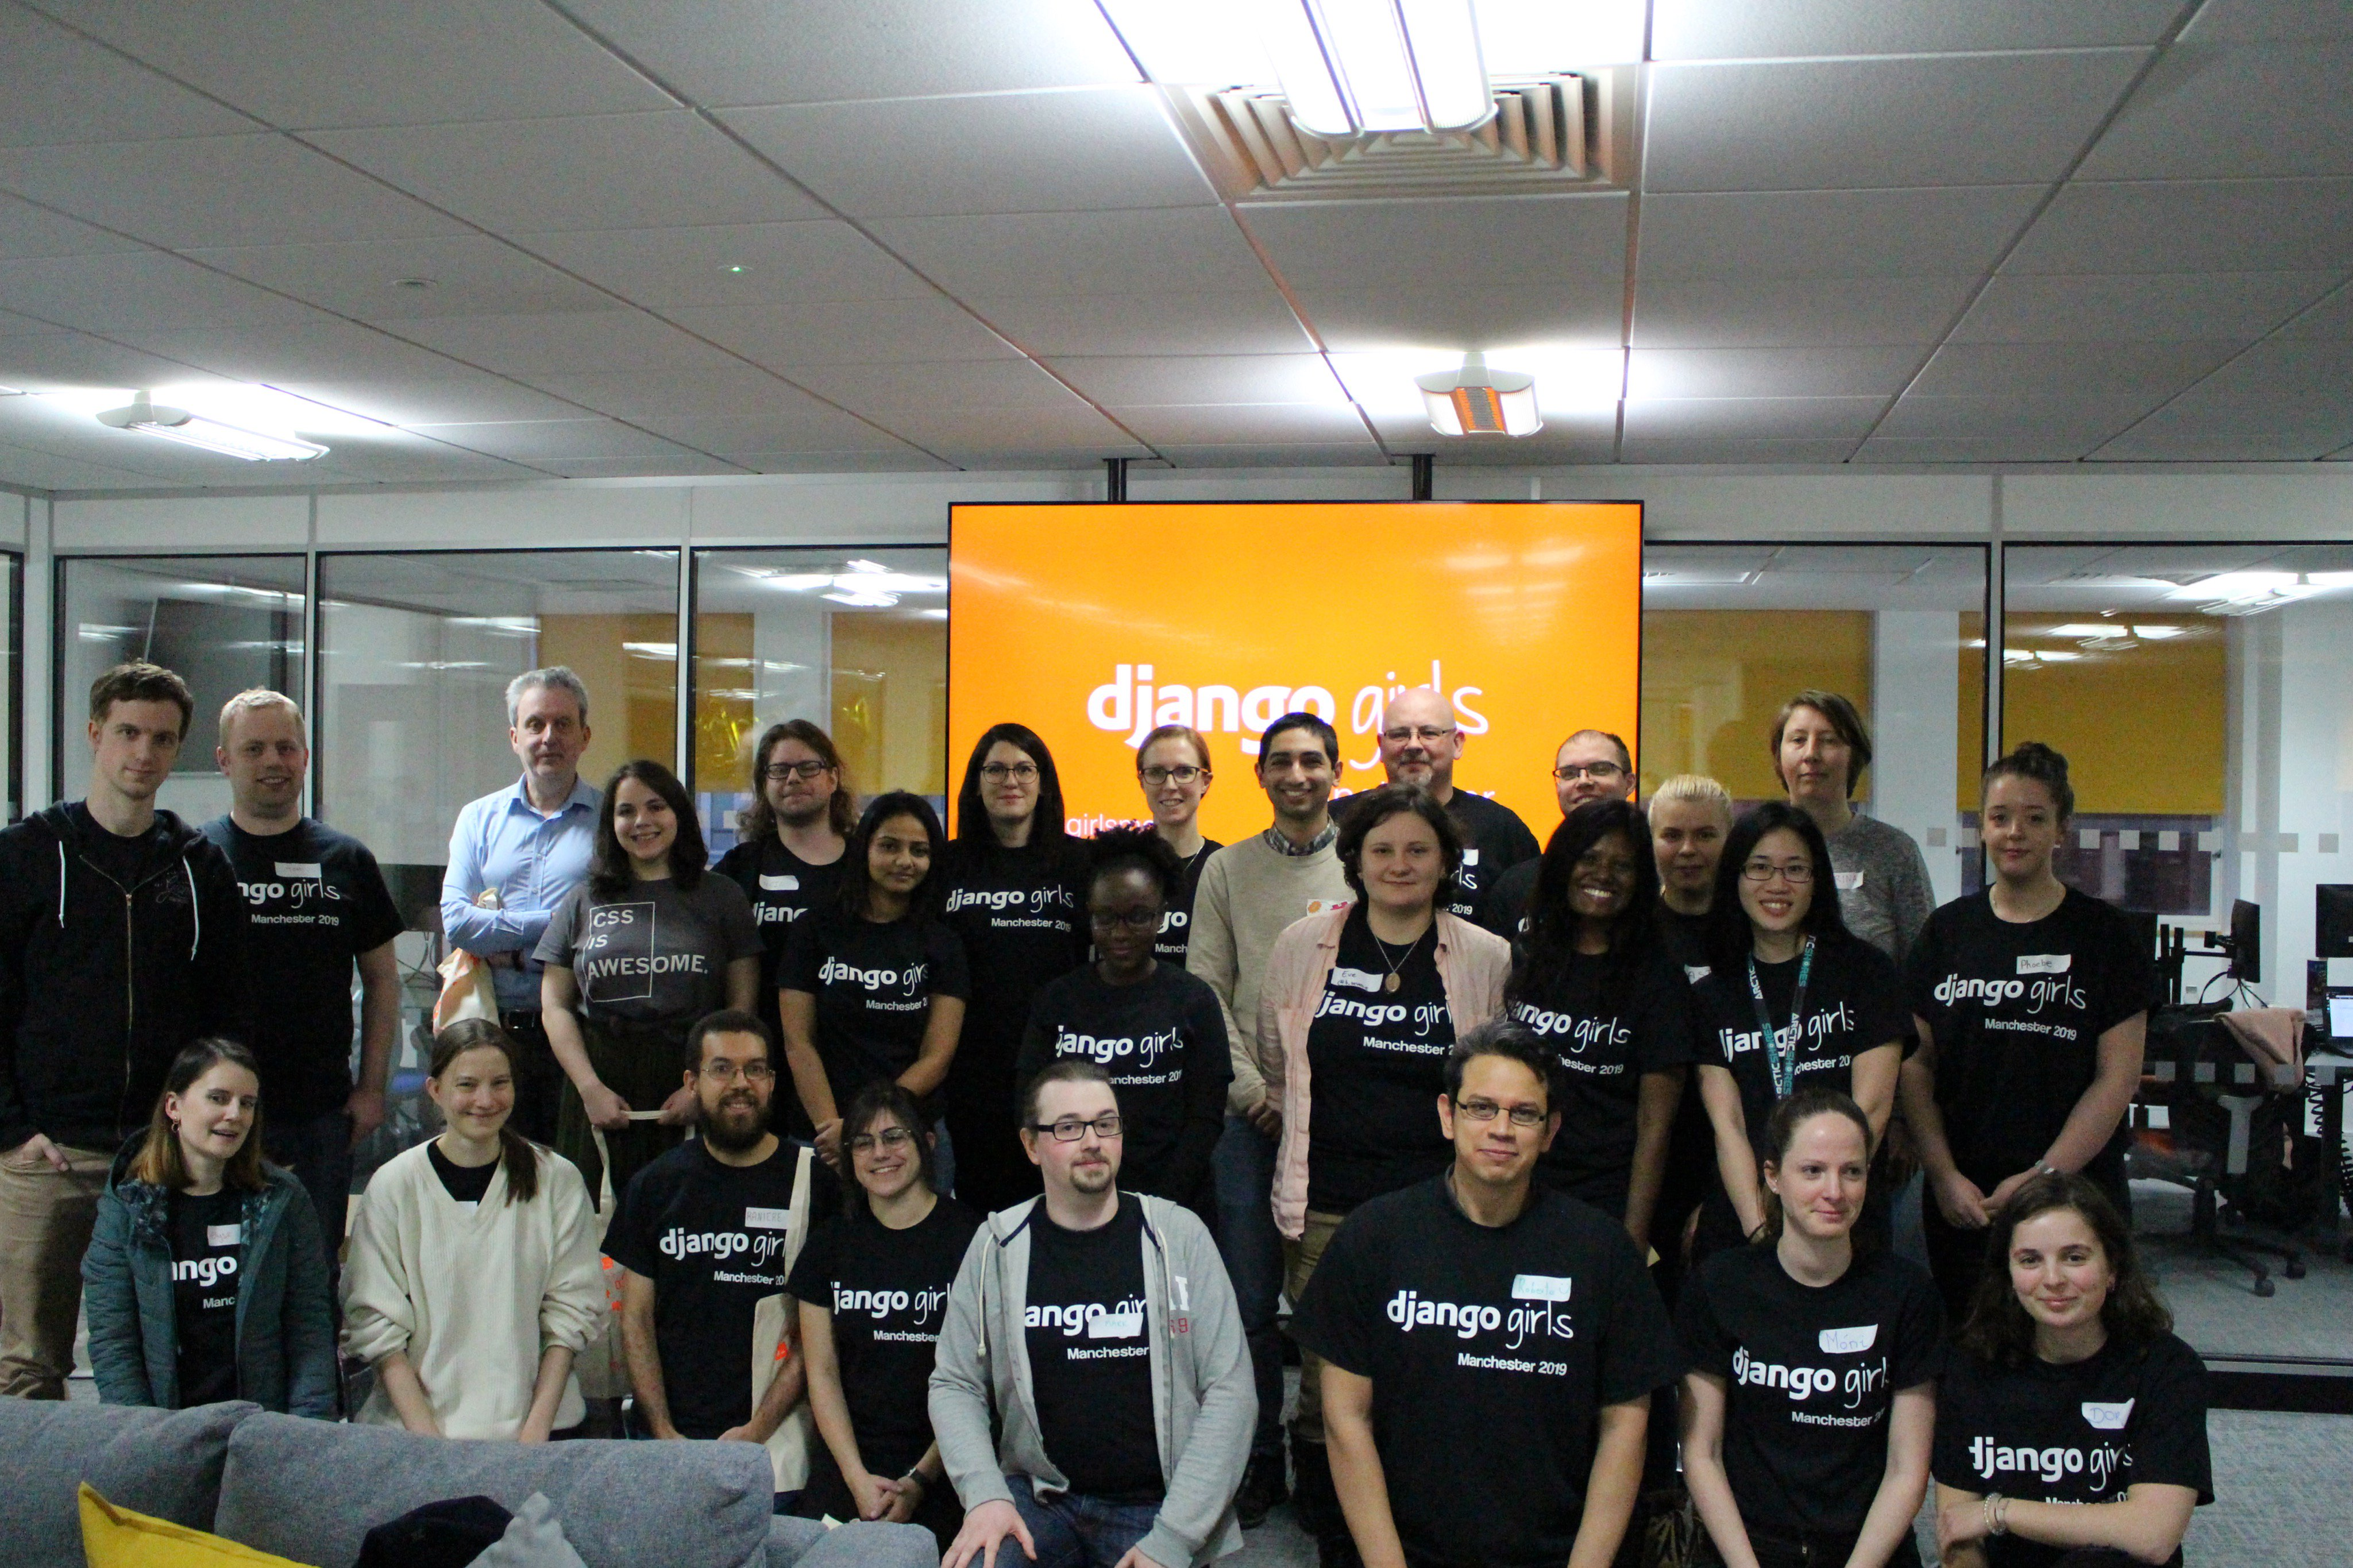
\includegraphics[width=.7\textwidth]{static/mcr_2019} \\
    \textbf{MANCHESTER 2019}
    \end{center}
\end{frame}

\begin{frame}
    \begin{center}
        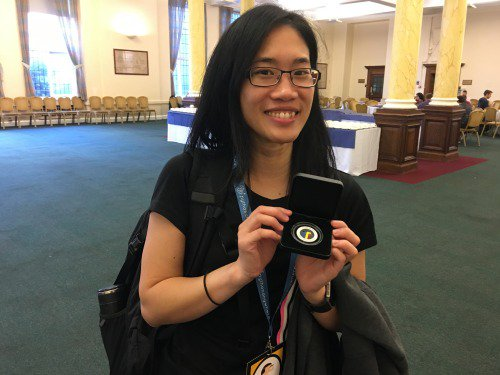
\includegraphics[width=.7\textwidth]{static/leona} \\
    \textbf{Leona @lwyso}
    \vspace{1cm}

    \scriptsize{\textbf{blog.djangogirls.org/post/172001842084/your-django-story-leona-so}}
    \end{center}
\end{frame}

\begin{frame}
    \begin{center}
    https://blog.djangogirls.org
    \end{center}
\end{frame}

\begin{frame}
    \begin{center}
    \textbf{\textcolor{orange}{TIPS}}
    \end{center}
\end{frame}

\begin{frame}
    \begin{center}
        \textbf{\textcolor{orange}{GAIN AS MUCH AS YOU CAN FROM YOUR COMMUNITY}}
    \end{center}
\end{frame}

\begin{frame}
    \begin{center}
        \textbf{\textcolor{orange}{GIVE BACK TO YOUR COMMUNITY}}
    \end{center}
\end{frame}

\begin{frame}
    \begin{center}
        \textbf{\textcolor{orange}{MEETUPS MEETUPS MEETUPS MEETUPS!}} \\
        \textbf{\textcolor{orange}{MEETUPS MEETUPS MEETUPS MEETUPS!}} \\
        \textbf{\textcolor{orange}{MEETUPS MEETUPS MEETUPS MEETUPS!}} \\
    \end{center}
\end{frame}

\begin{frame}
    \begin{center}
    \faTwitter \ @NikoletaGlyn \\
    \faInstagram \ nikoleta\_v3
    \end{center}
\end{frame}

\end{document}

